\chapter{Conception Fonctionnelle des Modules}

\section{Le Module d'Authentification}
Le pilier de la sécurité de l'application repose sur le service d'authentification. Il implémente les flux de connexion standard, l'inscription et la gestion des mots de passe. Il génère et valide les jetons JWT qui accompagnent chaque requête HTTP au sein de l'écosystème.

\begin{figure}[h!]
    \centering
    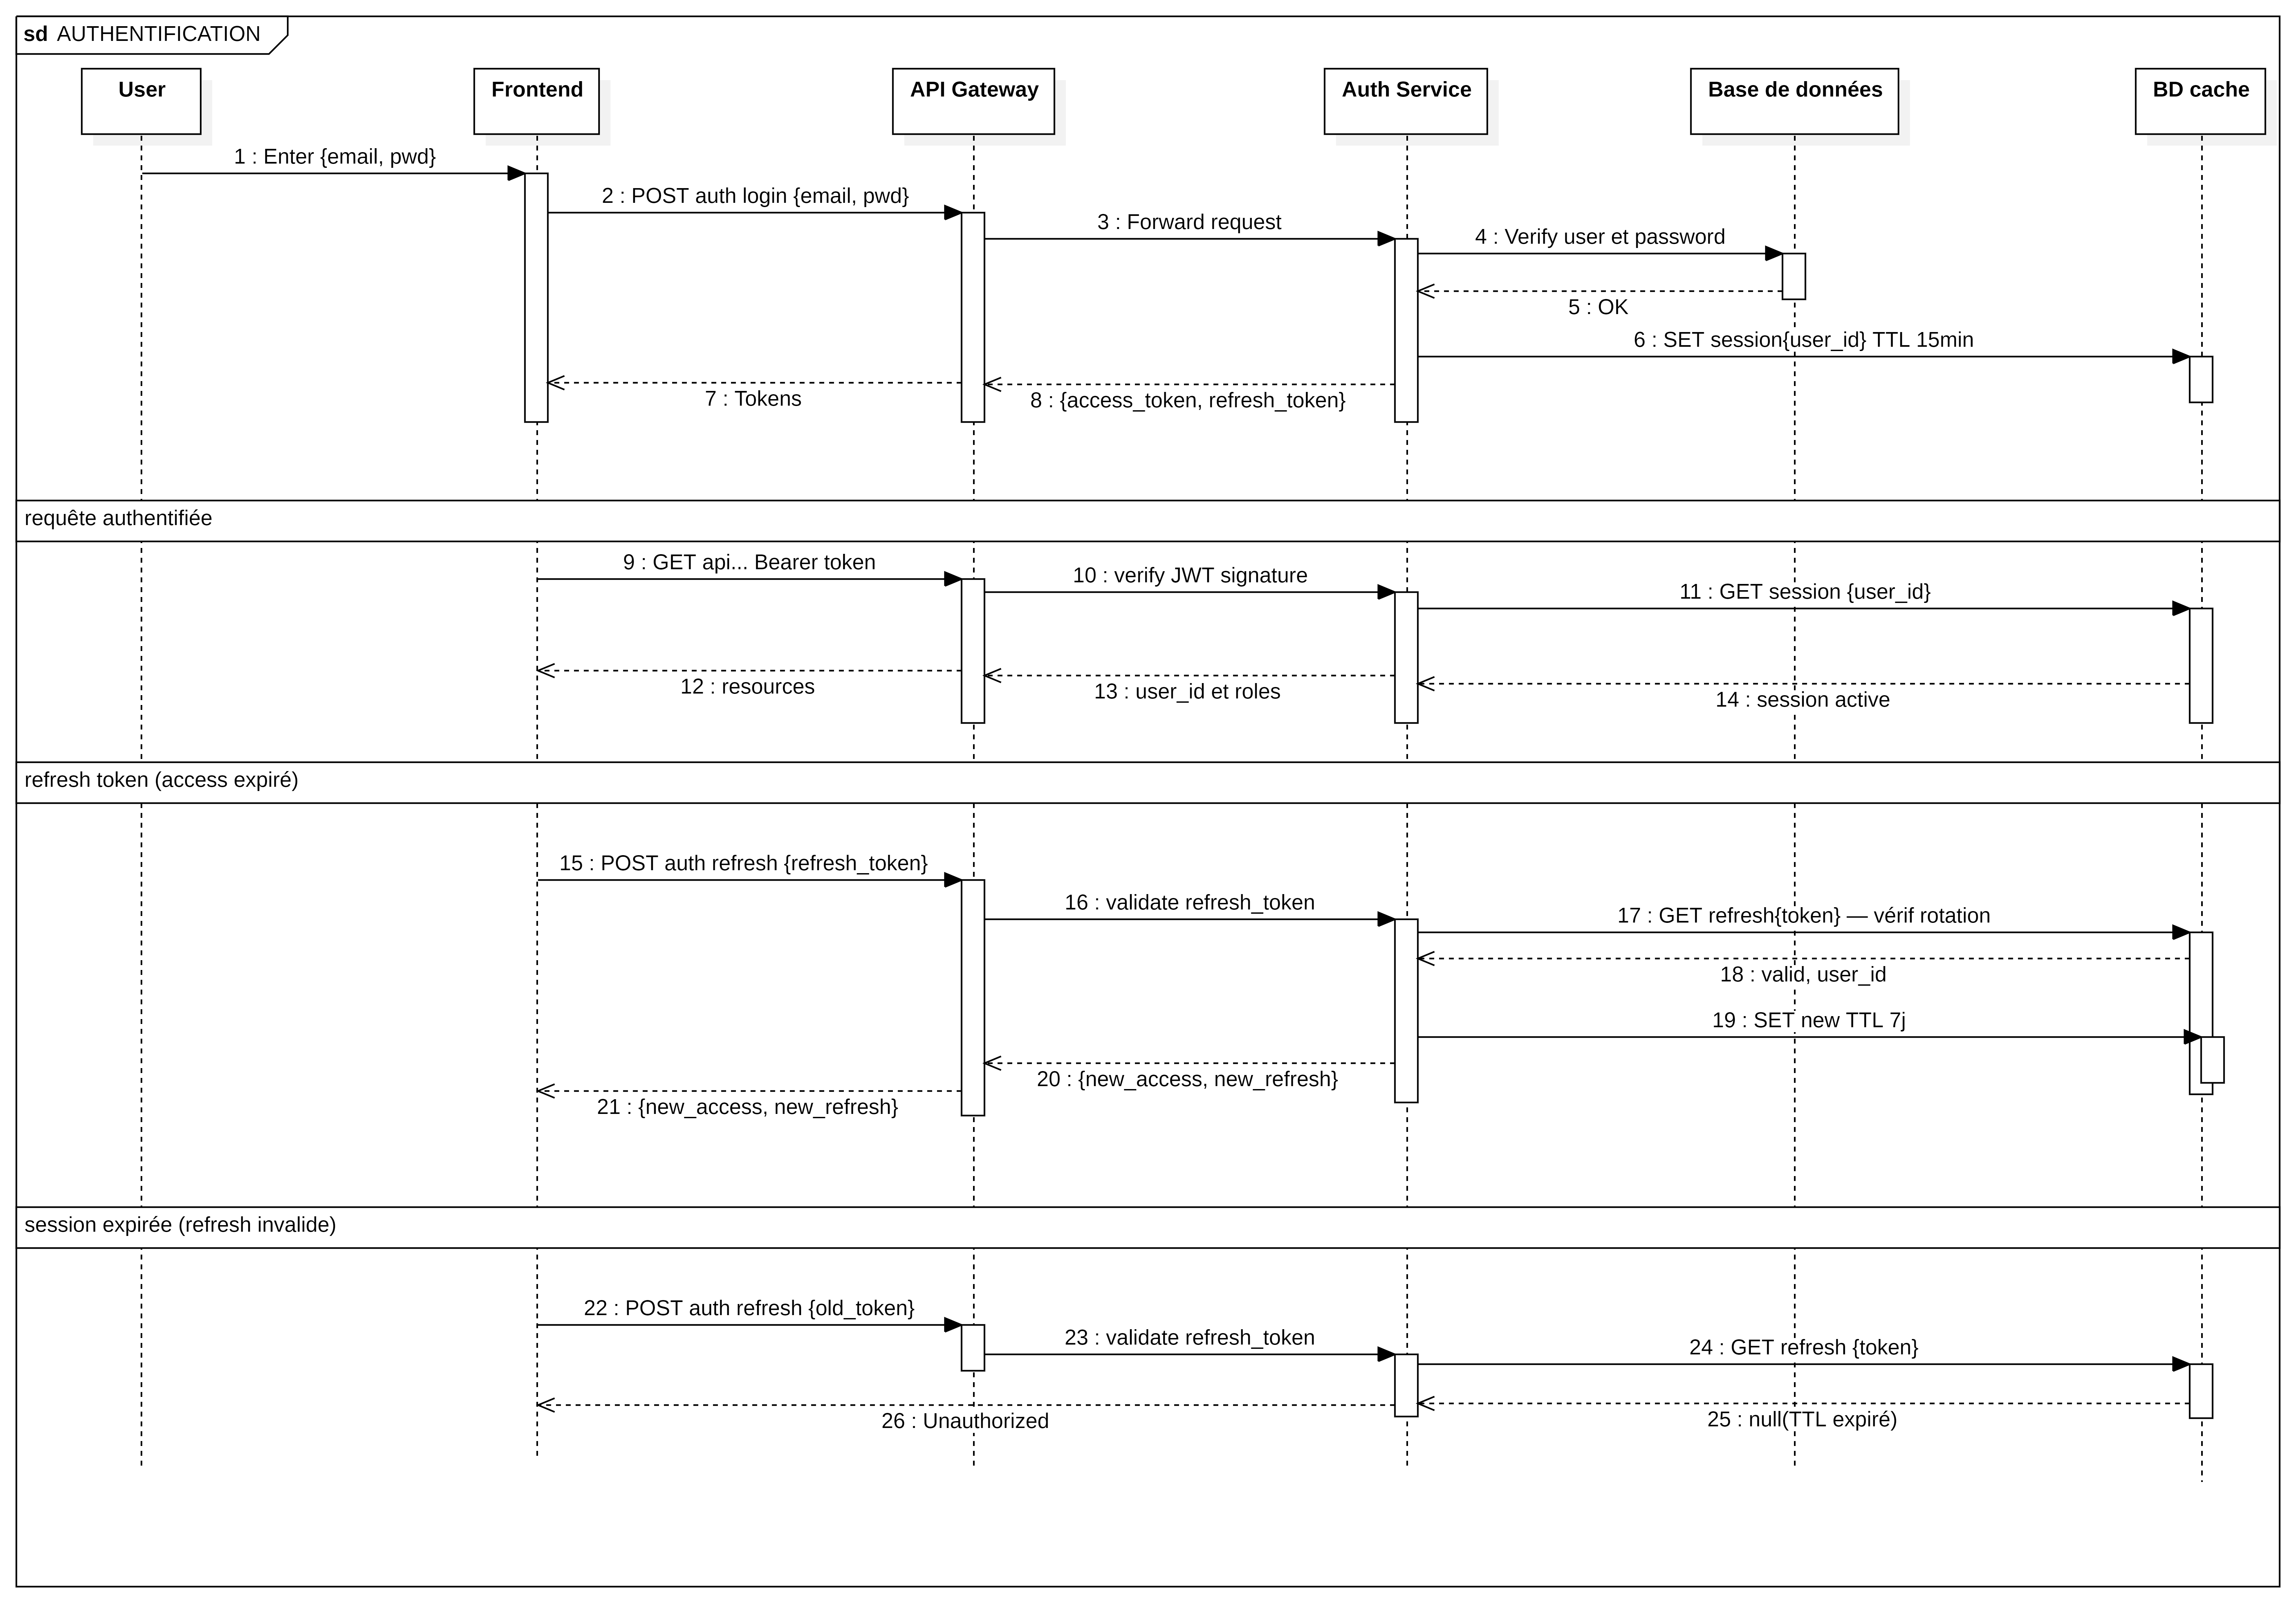
\includegraphics[max width=\textwidth, max height=0.4\textheight, keepaspectratio]{../AUTHENTIFICATION.png}
    \caption{Architecture du Module d'Authentification}
    \label{fig:mod_auth}
\end{figure}

\section{Le Module Learning Hub}
L'interface d'apprentissage, ou Learning Hub, est le point d'entrée quotidien de l'apprenant. La conception de ce module met l'accent sur la clarté visuelle et la progression pédagogique.

\begin{figure}[h!]
    \centering
    \includegraphics[max width=\textwidth, max height=0.4\textheight, keepaspectratio]{../LearningHub.png}
    \caption{Conception de l'Interface Learning Hub}
    \label{fig:mod_learning}
\end{figure}

Le flux d'apprentissage est dynamique. Selon les performances antérieures de l'étudiant analysées par le service Analytics, le système suggère automatiquement le chapitre ou la notion à réviser en priorité.

\begin{figure}[h!]
    \centering
    \includegraphics[max width=\textwidth, max height=0.4\textheight, keepaspectratio]{../Learning_Flow.png}
    \caption{Diagramme de séquence du Flux Pédagogique}
    \label{fig:mod_learning_flow}
\end{figure}

\section{Le Module d'Évaluation (Assessment)}
L'évaluation est l'un des processus les plus critiques. Du côté étudiant, l'interface doit être épurée, exempte de distractions et synchronisée avec le chronomètre officiel de l'examen. Du côté enseignant, l'interface propose des outils de révision et d'ajustement des notes suggérées par l'IA.

\begin{figure}[h!]
    \centering
    \includegraphics[max width=\textwidth, max height=0.4\textheight, keepaspectratio]{../Student_assessment.png}
    \caption{Interface d'Évaluation - Vue Étudiant}
    \label{fig:student_assessment}
\end{figure}

L'architecture de déroulement de l'examen assure la sauvegarde périodique des réponses de l'étudiant pour prévenir toute perte de données en cas de coupure de connexion, et verrouille l'environnement visuel.

\begin{figure}[h!]
    \centering
    \includegraphics[max width=\textwidth, max height=0.4\textheight, keepaspectratio]{../Teacher_assessment.png}
    \caption{Diagramme de séquence du Suivi des Évaluations}
    \label{fig:teacher_assessment}
\end{figure}

\begin{figure}[h!]
    \centering
    \includegraphics[max width=\textwidth, max height=0.4\textheight, keepaspectratio]{../Examen.png}
    \caption{Diagramme de séquence de la Composante Examen}
    \label{fig:examen_detail}
\end{figure}
